\subsection{GUI}
\label{subsec:gui}

The GUI \texttt{weviation.py} is made using wxPython, which is a library wrapper to create interfaces.
The interface allows users to have flexibility in calculating the weight by having more options.
The components to be calculated can be chosen, the unit for the input and output  parameters can be changed, the output can be exported as a text file and a bar chart is present.
The GUI is divided into three main sections: input window (left), output text window (middle), output visual window (right); see Figure~\ref{fig:gui1}.

The first step in creating a GUI is to come up with a simple layout.
A simple layout means having sections which are the same size, as less size configuration is needed, and therefore the three windows are the same in size.
The next step is the tabpanel in the left section, which is created using command called \texttt{wx.Notebook}.
Once a tab for each method is in place, the component selection and parameter value input are created with unit and type selection.
When the user hits the calculate button the program will first look at which methods are selected (in the bottom of the left section) and then look at which component(s) is selected and extract the non-empty values from the white text space, called text control (using wx.TextCtrl), and place them into a dictionary.
Similar to the black box (see Section~\ref{subsec:blackbox}) the functions from \texttt{methods.py} are imported.
All extracted values from the text control are converted to imperial units if unit selection is not imperial, since the functions expect values to be in imperial, and are put into the functions.
The results of those functions are put into a dictionary per method and are used for the output- and visual  window.

The output window section (middle) is essentially a large text control panel and it set to read-only to prevent alteration of the output values.
Before the values are printed in the text control, the name of the value and unit are added to it.
The text in the window is appended everytime the user hits calculate button and in order to clear the output window, the clear button can be pressed, which will set the value of the text control to "", which means empty.

In the visual output window (right) the dictionaries are used.
Similarily to the left section, tabs are used to display each pie chart and one bar chart.

\begin{figure}[ht]
\centering
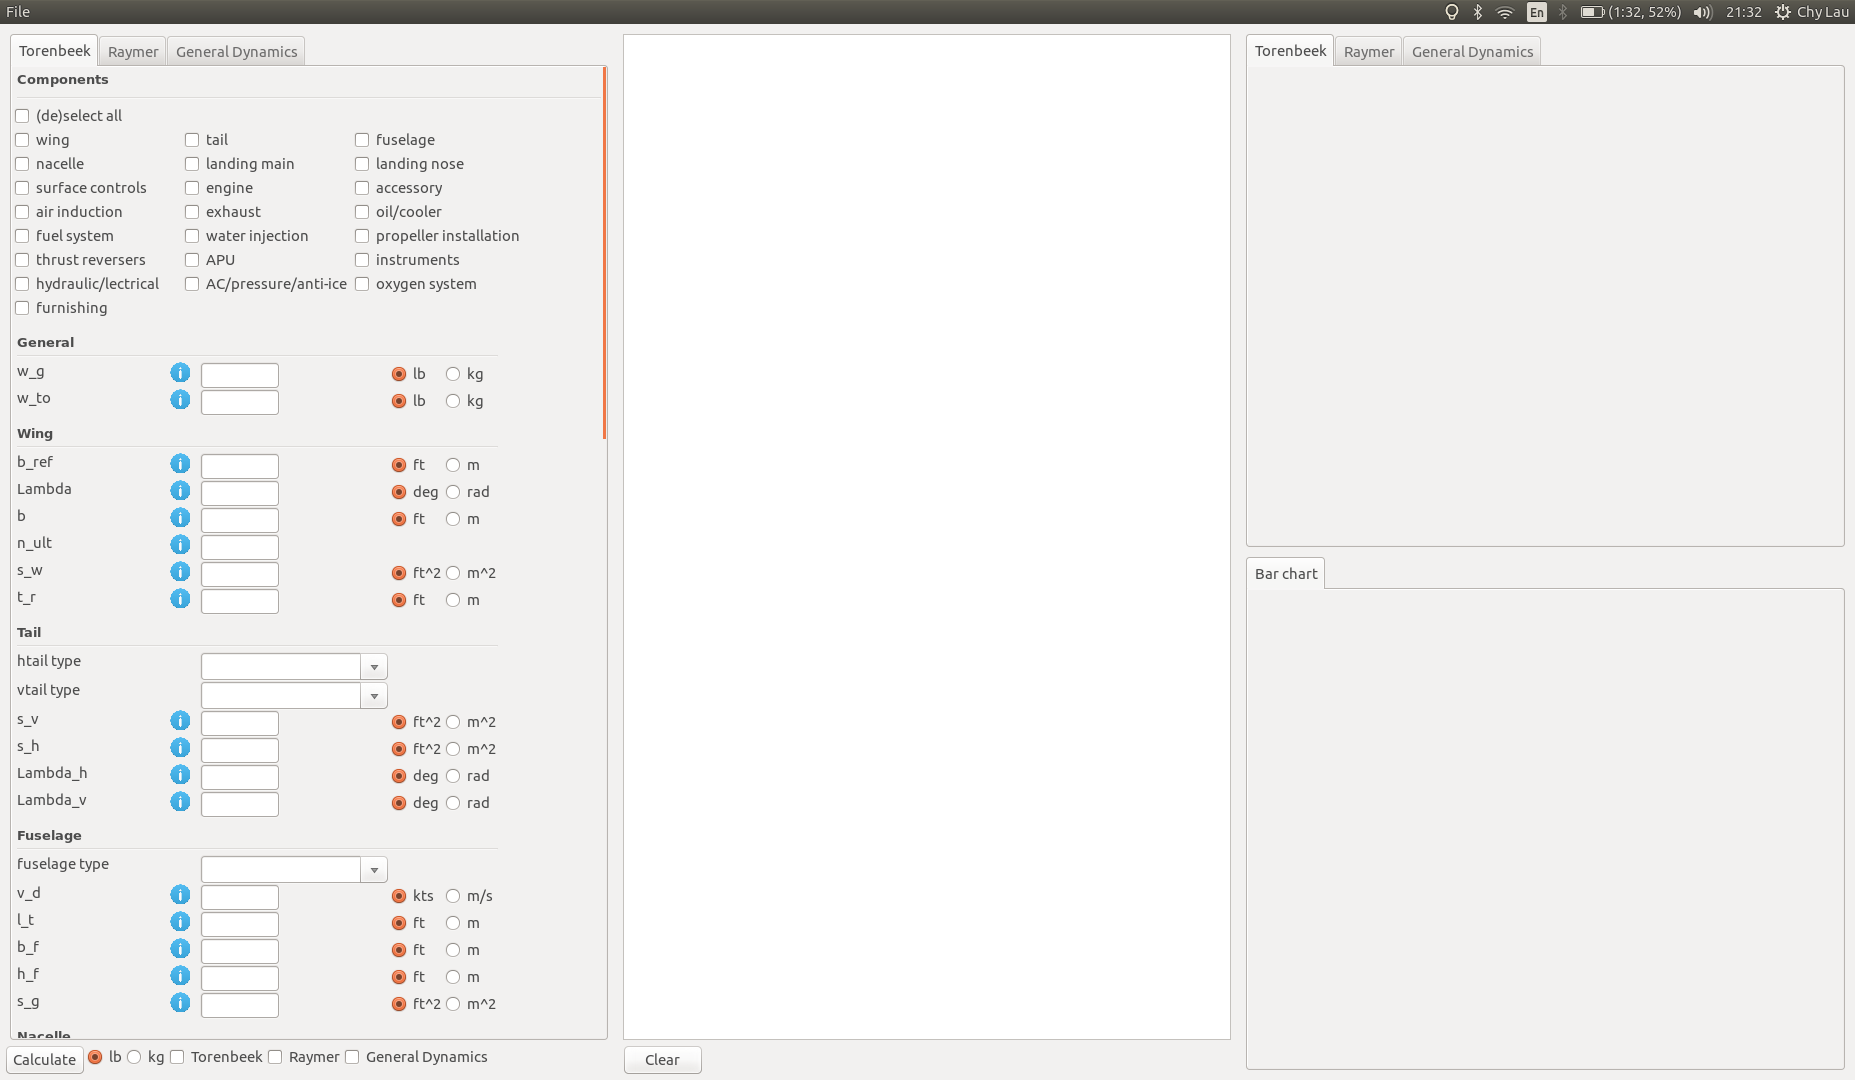
\includegraphics[width=1\textwidth]{image/gui_startup.png}
\caption{GUI on startup.}
\label{fig:gui1}
\end{figure}

In the file menu at the top, several options can be selected: load XML file, export to XML and export to text.
The load XML file option calls \texttt{parse.py} and sets the text control and combo box (type selection) to the parsed value.
Exporting to a XML/text file is done in the gui file and are saved as \texttt{output.xml} and \texttt{output.txt} for XML and text respectively.


